\section{Support Aggregation}
\label{sec:data-aggregation}
Namespace should also be designed to support content aggregation, so that applications, at API level, can subscribe to a specific prefix and expect all relevant data below it.
Thus organization the hierarchal name is crucial, given the hierarchy design determines the pattern of aggregation.  

We start determining the hierarchy by making observation that in most cases \textit{effective scope} and \textit{command identifier} are finer granularity of \textit{data type} and \textit{capability}.
Hence the latter two should be at front of the former two.
Then we consider aggregation apporach can benefit application most. 

\begin{figure}[!h]
    \centering
    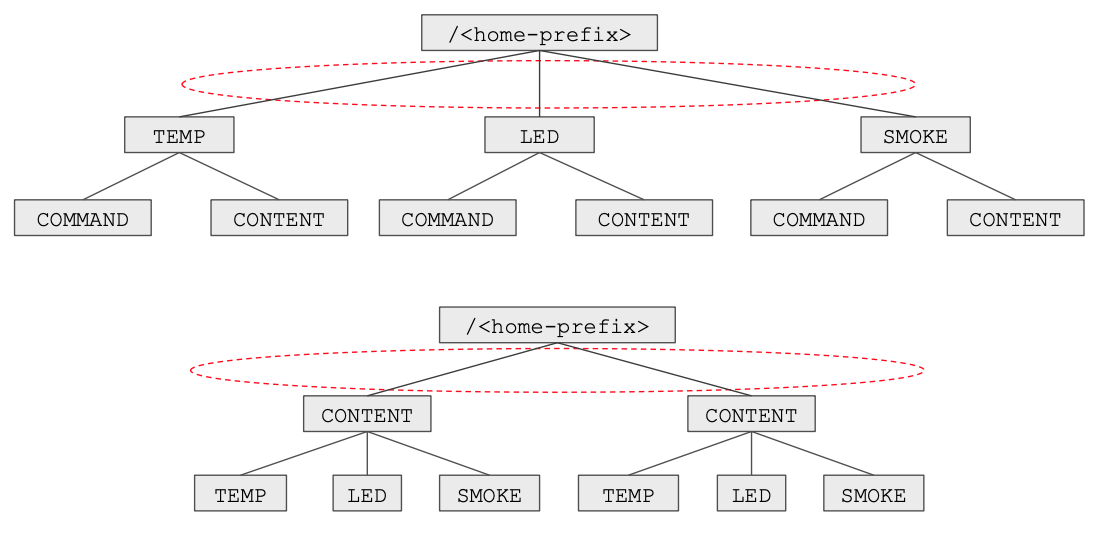
\includegraphics[width=0.5\textwidth]{comparison}
    \caption{Aggregation Approaches Comparison}
    \label{fig:aggregation-comparison}
\end{figure}

Another important observation made is \textit{capability} and \textit{effective scope} are more expressive and providing more data collection dimensions than the other two.
More expressive components should be at smaller depth inside the nametree, to avoid communication overhead of Pub/Sub.
An example is given in Fig~\ref{fig:aggregation-comparison} with three \textit{capability} are invovled. 
One have three dimensiosns of freedom to access namespace from \textsl{/<home-prefix>} when \textit{capability}'s position is upper than \textit{data type}.
In contrast, the other way of aggregation only provide two dimensions of freedom for namespace accessing at the entry point.
In the first organization, received data of subscription on the first depth are either commands or content.
However, data are less guessable when the same subscription happens on the second organization since \textit{capability} has numerous types and more expressive.
Same analysis applies on \textit{effective scope} and \textit{command identifier} situation, and \textit{effective scope} prevails in our application scenarios.

Finally we get the hierarchy which benefits content aggregation most: \textsl{/<home-prefix>/<capability>/<data-type>/<effective-scope>/<data-id>}.
This order also better fit the functionality separation feature in Section~\ref{sec:separation}.
We argue this hierarchy is the outcome of current NDN-Lite applcation needs of accessing namespace with maximized freedom, and this hierarchy may change if applcation needs shift in future.